% Two-axis map for Ch12 ("Beyond One Agent, One Tool") — the Tools & Orchestration spine.
% Standalone TikZ; compiled by `book-scaffold build-figures` via pdflatex -> pdftocairo -> SVG.
% Horizontal = capability (what to expose; subtract-first default). Vertical = coordination
% (how many isolated windows: one agent -> sub-agent primitive -> multi-agent topology).
\documentclass[tikz,border=4mm]{standalone}
\usepackage{tikz}
\usetikzlibrary{positioning, arrows.meta, calc}

\begin{document}
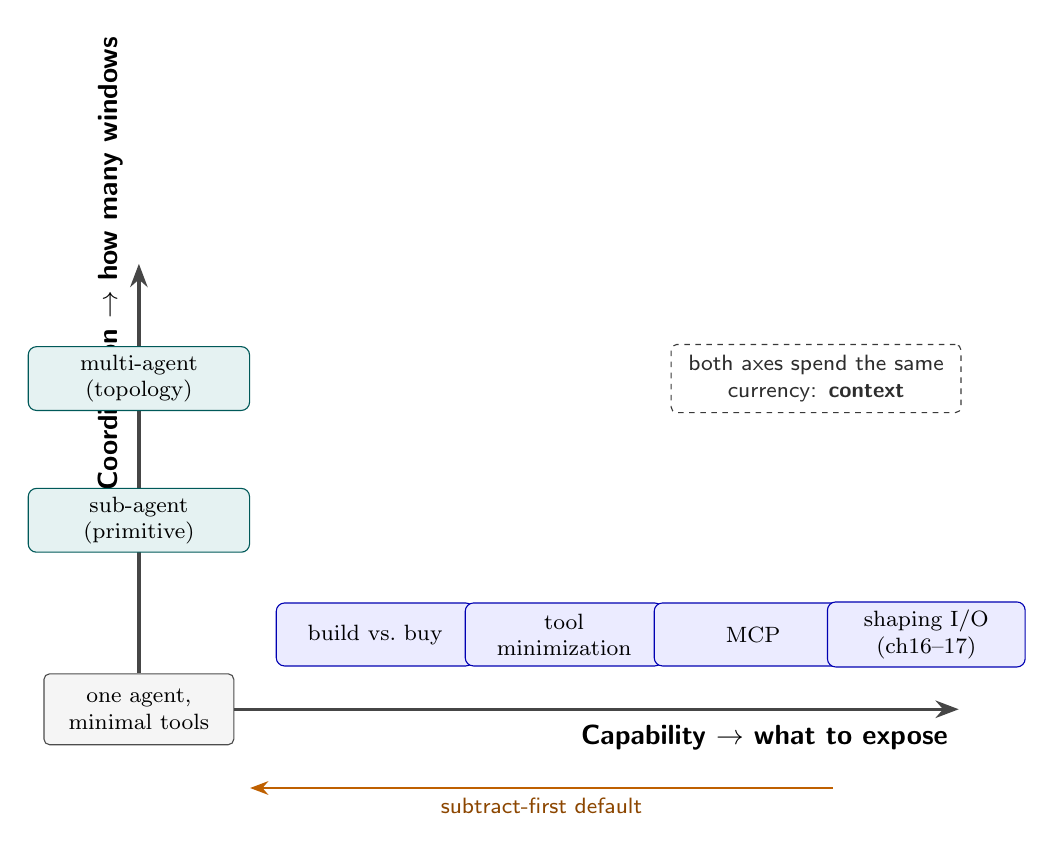
\begin{tikzpicture}[
  font=\sffamily,
  ax/.style={-Stealth, very thick, draw=gray!55!black},
  capbox/.style={draw=blue!70!black, fill=blue!8, rounded corners=3pt, align=center,
    text width=2.3cm, minimum height=0.8cm, inner sep=3pt, font=\footnotesize},
  coordbox/.style={draw=teal!70!black, fill=teal!10, rounded corners=3pt, align=center,
    text width=2.6cm, minimum height=0.8cm, inner sep=3pt, font=\footnotesize},
  subarr/.style={-Stealth, thick, draw=orange!75!black}
]

% origin
\node[draw=gray!60!black, fill=gray!8, rounded corners=2pt, align=center,
  text width=2.2cm, minimum height=0.9cm, inner sep=3pt, font=\footnotesize] (orig) at (0,0)
  {one agent,\\minimal tools};

% --- horizontal axis: capability ---
\draw[ax](orig.east) -- ++(9.2,0)
  node[below=2pt, font=\sffamily\bfseries, anchor=north east] {Capability $\rightarrow$ what to expose};
\draw[subarr] ($(orig.east)+(7.6,-1.0)$) -- ($(orig.east)+(0.2,-1.0)$)
  node[midway, below, font=\sffamily\footnotesize, text=orange!55!black] {subtract-first default};

\node[capbox](c13) at (3.0,0.95) {build vs.\ buy};
\node[capbox](c14) at (5.4,0.95) {tool\\minimization};
\node[capbox](c15) at (7.8,0.95) {MCP};
\node[capbox](c16) at (10.0,0.95) {shaping I/O\\(ch16--17)};

% --- vertical axis: coordination ---
\draw[ax](orig.north) -- ++(0,5.2)
  node[left=2pt, rotate=90, anchor=south, font=\sffamily\bfseries] {Coordination $\rightarrow$ how many windows};
\node[coordbox](sa) at (0,2.4) {sub-agent\\(primitive)};
\node[coordbox](ma) at (0,4.2) {multi-agent\\(topology)};

% corner note
\node[draw=gray!45!black, dash pattern=on 2pt off 2pt, rounded corners=2pt, align=center,
  text width=3.4cm, inner sep=4pt, font=\sffamily\footnotesize, text=gray!35!black]
  at (8.6,4.2) {both axes spend the same\\currency: \textbf{context}};

\end{tikzpicture}
\end{document}
